\documentclass[paper.tex]{subfiles}

\begin{document}
\section{Introduction}

\begin{figure}[h]
    \centering
    \begin{subfigure}[b]{0.3\textwidth}
        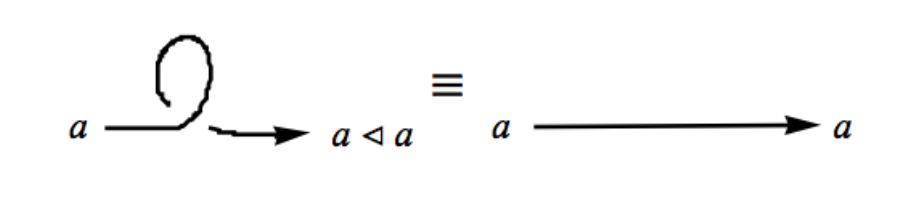
\includegraphics[width=\textwidth]{figures/R1}
        \caption{R1}
    \end{subfigure}
    ~ %add desired spacing between images, e. g. ~, \quad, \qquad, \hfill etc.
      %(or a blank line to force the subfigure onto a new line)
    \begin{subfigure}[b]{0.3\textwidth}
        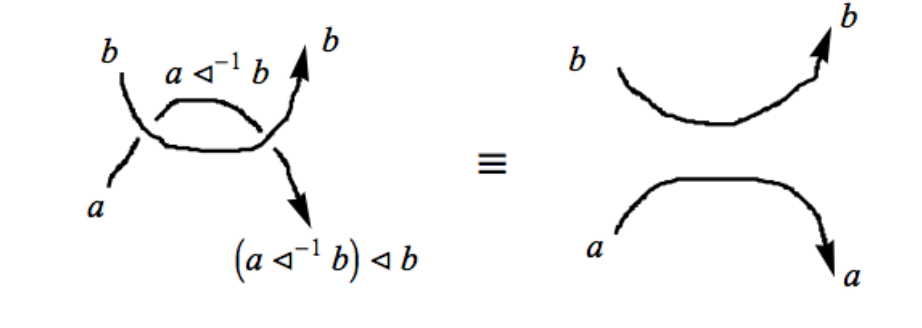
\includegraphics[width=\textwidth]{figures/R2}
        \caption{R2}
    \end{subfigure}
    ~ %add desired spacing between images, e. g. ~, \quad, \qquad, \hfill etc.
    %(or a blank line to force the subfigure onto a new line)
    \begin{subfigure}[b]{0.3\textwidth}
        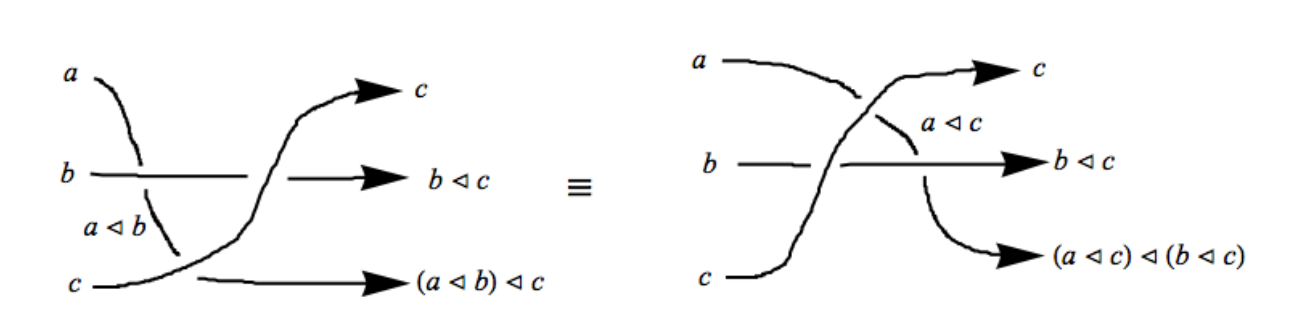
\includegraphics[width=\textwidth]{figures/R3}
        \caption{R3}
    \end{subfigure}
    \caption{The quandle axioms are chosen such that quandle colorings are naturally diagram invariant. Figures reproduced from~\cite{Cusick}}\label{fig:quandle_axioms}
\end{figure}




\subsection{Involutary Quandle}
In this paper we concern ourselves with \textbf{Involutory Quandles}. An \textbf{involutory quandle} is any set $K$ equiped with a binary operation $\uc$ that satisfies $3$ axioms:

\begin{equation}
	x \uc x = x
\end{equation}
\begin{equation}
	x \uc (x \uc y) = y \\
\end{equation}
\begin{equation}
	x \uc (y \uc z) = (x \uc y) \uc (x \uc z) \\
\end{equation}

These equations can be though of a symbolic representations of Reidemeister moves. $(1)$ corresponds to the Type I Reidemeister move, $(2)$ corresponds to the Type II Reidemeister move, and $(3)$ corresponds to the Type III Reidemeister move. (See Fig)

\subsection{Alexander Quandle}

The \textbf{Alexander Quandle} is defined as:

$$ x \uc y = ty + (1 - t)a $$

$t$ is usually a free variable in $\mathbb{C}$ however for this paper we consider a special case of the Alexander Quandle:

$$ x \uc y = qy + (1 - q)a $$

where $q$ is a free variable in $\mathbb{Z}_n$. The reasons for this will be made clear when we consider the relationship between the Alexander Quandle and coloring.

\subsection{Dihedral Quandle}
The \textbf{Dihedral Quandle} is defined as:

$$x\uc y = 2x - y$$

it is a special case of the Alexander quandle when $t$ is evaluated at $-1$.

\subsection{Coloring}

We say that a knot $K$ is $Z_p$ colorable if given an prime $p > 2$ every strand in the projection of $K$ can be labeled using numbers $0$ to $p-1$, with at least 2 of the labels distinct so that at each crossing we have:

$$ 2x - y - z = 0 \mod p $$

(TODO: Cite FinalPaper.pdf)

\subsection{Quandle Coloring}

(TODO: Complete the description)
We say that a knot is $Z_{p,q}$ colorable if for some unit $q \in \mathbb{Z}_p$ there is a labeling of strands so that

\end{document}
